\chapter{Matériel et parallélisme}
\label{sec:materiel}
%Nous avons a ce stade un aperçu du type de calcul a effectuer, essayons d'estimer . 
%De plus, les simulations cosmologiques ont pour principal défi de simuler d'important volume d'espace avec la meilleure résolution possible.

Le défis des simulations de la réionisation est qu'elles doivent simuler un volume d'univers suffisant grand pour être représentatif de la variance cosmique( $\approx 100$ Mpc selon \cite{iliev_cosmological_2006}) tout en résolvant la formation stellaire (échelle $<1$ pc).
En première approximation, il nous faudrait donc échantillonner un tel volume par $\left( \frac{100Mpc}{1pc} = 10^7 \right) ^3 = 10^{21}$ éléments.
Ce qui est totalement impossible à l'heure actuelle.
%Nous verrons dans la prochaine partie que nous sommes encore loin de pouvoir résoudre la formation stellaire dans ce type de simulations. %TODO ref
Nous avons vu que l'amélioration de certain algorithme (passage de grilles fixe a grille adaptative, intégration du potentiel plutôt que somation Ncorps directe, etc... cf chapitre \ref{ch:introduction}) a permis d'augmenter significativement la taille des simulations à puissance de calcul identique, mais le principal facteur limitant reste au niveau du matériel.

\subsection{Loi de Moore et simulations}
La loi de Moore \citep{moore1965cramming} propose un doublement du nombre de transistor par circuit intégré tout les 18 mois environs. (Fig \ref{fig:moore})
Comme la puissance de calcul est étroitement liée a cette évolution, la taille -- le nombre d'éléments de résolution -- des simulations, suis également cette croissance exponentielle (Fig. \ref{fig:taillesimu}).

\begin{figure}[bth]
        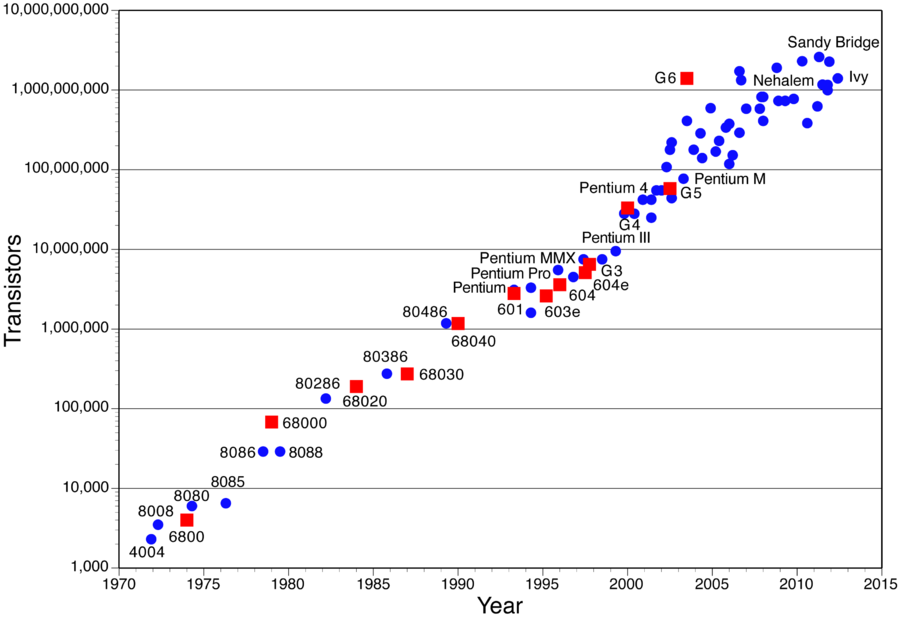
\includegraphics[width=.95\linewidth]{img/02/moorelaw.png} 
        \caption[Loi de Moore]{Nombre de transistor par processeur en fonction du temps ou loi de Moore}
 		\label{fig:moore}
\end{figure}

\begin{figure}[bth]
        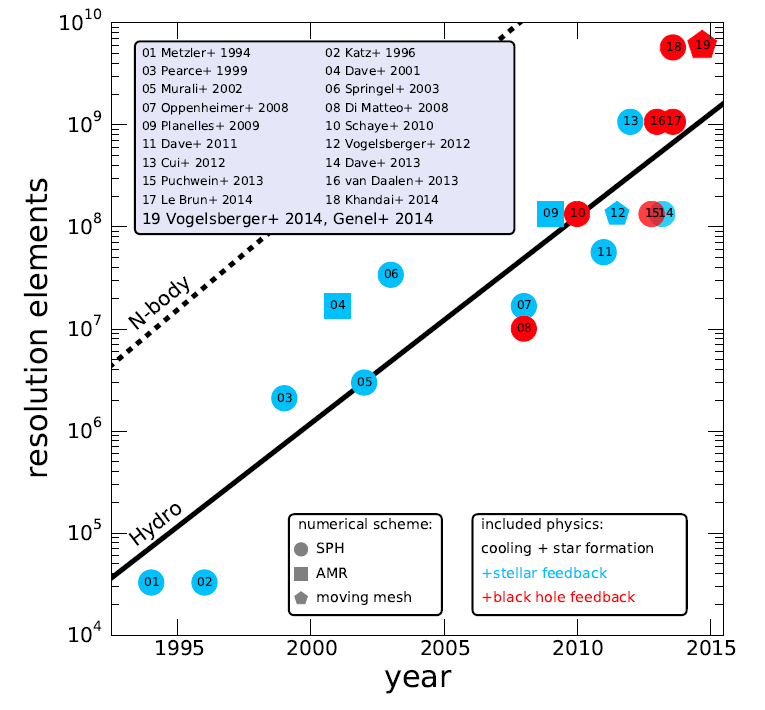
\includegraphics[width=.95\linewidth]{img/02/figure_simulations_with_time.png} 
        \caption[Évolution de la taille des simulations]{Tailles des simulations en fonction du temps.
        Il existe un lien direct avec la loi de Moore.
        Image illustris}
 		\label{fig:taillesimu}
\end{figure}


\subsection{Principes de parallélisation}

Comme on ne peux pas créer des processeurs aussi gros que ce que l'on le souhaite, la technique utilisée pour continuer à augmenter la puissance de calcul, consiste à en utiliser plusieurs en parallèle.
Dans le cas des simulation cosmologique, la parallélisation est effectué en découpant l'espace à simuler en un certain nombre de sous domaines chacun associé à une unité de calcul.
Comme chaque sous domaine n'est pas isolé, mais appartient au même ensemble, les domaines vont devoir communiquer entre eux sur l'état de leurs voisin.
Nous verrons en détail comment est effectué ce découpage dans la section \ref{sec:parasoft}.
Mais voyons d'abord un aperçut des contraintes techniques de la parallélisation.
Il existe différent type de parallélisation définis par la taxonomie de Flynn \citep{Flynn:1972:COE:1952456.1952459}: 

\begin{itemize}
\item SISD Single Instructions on Single Data.
Aucun parallélisme, exécution d'une unique série d'instructions sur un unique flux de données.

\item SIMD Single Instructions on Multiple Data.
Exécution d'une unique série d'instructions sur différents flux de données.
C'est le principe de fonctionnement des GPU.

\item MISD Multiple Instructions on Single Data 
Exécution de différentes série d'instructions sur un seul flux de données.

\item MIMD Multiple Instructions on Multiple Data.
Exécution de différentes série d'instructions sur différents flux de données.
C'est l’architecture la plus utilisée aujourd'hui, et celle qui nous intéresse ici.
Le type MIMD est lui même découpé en deux sous ensembles : 

\begin{itemize}
\item On dit que la mémoire est \textit{distribuée} quand les processus ont leurs propres espaces mémoires dédiés.
Les principales machines que j'ai pu rencontrer utilise un modèle MIMD à mémoire distribuée.

\item On dit que la mémoire est \textit{partagée} quand plusieurs processus ont accès au mème espace mémoire.
\end{itemize}
\end{itemize}

Il existe plusieurs niveau de parallélisation, au niveau matériel.
Par exemple, un processeur actuel dispose de plusieurs cœurs, capable de géré chacun un processus (voir 2 dans le cas de l'hyperthreading).
Il est possible d'avoir plusieurs processeur au sein d'un même ordinateur.
Et il est possible d'utiliser conjointement plusieurs ordinateurs.
Ce qui nous mène à la notion de centre de calcul.

\subsection{Les calculateurs}

La production de simulation cosmologique à haute valeur scientifique se fait sur des centres de calcul.
A la manière d'un télescope pour les observateurs, les supercalculateur sont les outils principaux des simulateurs.
Et a la manière des plus gros télescopes, ces calculateurs sont gigantesques.
La figure \ref{fig:titan} présente le calculateur TITAN du Oak Ridge Leadership Computing Facility sur lequel ont été exécutées les simulations CODA \citep{ocvirk_cosmic_2015}.
En novembre 2015, TITAN a été classé deuxième plus puissant calculateur au monde selon le cite top500.org (cf \ref{tab:top500}), il est aujourd'hui quatrième.

\begin{figure}[bth]
        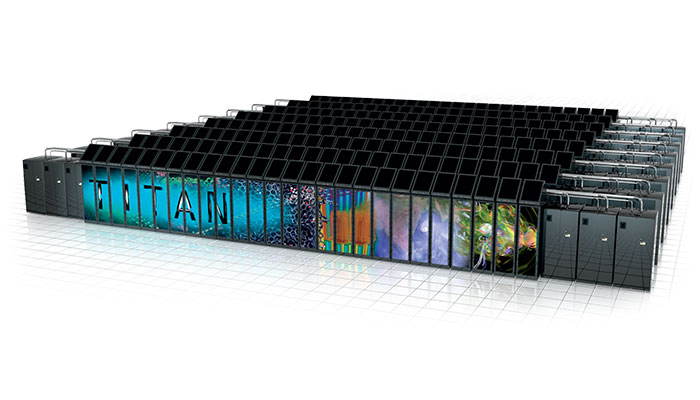
\includegraphics[width=.95\linewidth]{img/02/titan.jpg} 
        \caption[Titan]{Supercalculateur Titan OLCF.
        La calculateur sur lequel ont été exécutés les simulations CODA}
 		\label{fig:titan}
\end{figure}

\begin{table}[bth]
\begin{tabular}{ l l l l }
\hline 
Système & Pays & nb de cœurs & TFlop/s (peak) \\
\hline 
Sunway TaihuLight & Chine & 10,649,600 & 125,435.9 \\ 
Tianhe-2  & Chine & 3,120,000 & 54,902.4 \\ 
Piz Daint  & Suisse & 361,760 & 25,326.3 \\ 
Titan  & États unis & 560,640 & 27,112.5 \\ 
Sequoia  & États Unis &1,572,864 & 20,132.7 \\ 
\end{tabular} 
\caption{Les 5 super calculateurs les plus puissants du top500 de Juin 2017, source : www.top500.org}
\label{tab:top500}
\end{table}

Ce type de calculateur est composé d'un certain nombre de nœud qui communique entre eux par l'intermédiaire d'un réseau.
Un nœud est un élément conceptuellement proche d'un ordinateur personnel puisqu'il dispose d'une carte mère, avec un (ou plusieurs) \ac{CPU}, de la mémoire RAM, un \ac{SSD}/\ac{HDD} et parfois un \ac{GPU}.
D'une manière générale, plus des composants sont physiquement éloignés, plus leurs communications seront lente (cf \ref{tab:debits}).
La quantité d'information passant par une interface représente un certain coup et on cherchera à minimiser ce coup en optimisant le transfert des données à différents niveaux.

\begin{table}
\begin{tabular}{ l l }
\hline 
Interface  & Débit théorique \\
\hline 
Cache L1 & $\approx$ 700Go/s \\
RAM & $\approx$ 20 Go/s \\ 
PCIE 16x & $\approx$ 16 Go/s \\
InfiniBand & $\approx$ 5 Go/s \\
SSD & $\approx$ 600 Mo/s \\
HDD & $\approx$ 100 Mo/s
\end{tabular} 
\caption{Ordre de grandeur des débits théorique des différentes interface rencontrées lors de l'exécution d'un code HPC.
On cherchera à optimiser les communications utilisant les interfaces les plus lentes.}
\label{tab:debits}
\end{table}

%Les cœurs au sein d'un même CPU pourront communiquer entre eux de faible quantité de données par l’intermédiaire du cache, ou en passant par la RAM pour les volumes plus importants.

%Proche d'un ordinateur personnel un nœud est composé d'une carte mère sur laquelle est relié entre autres, un ou plusieurs processeurs (CPU), une certaine quantité de mémoire RAM et parfois une carte graphique (GPU)
%Chaque CPU dispose d'un certain nombre de cœurs, et chaque cœurs est capable d'exécuter un certain nombre de processus ou thread (généralement 1, parfois 2 dans le cas de l'Hyperthreading)

%Une fois les processus et les domaines identifiés il existe différentes facons de faire dialoguer les processus entre eux.
%La principale distinction viendra généralement de si les threads sont exécutés par un meme noeud ou non.
%
%, cad par exemple que si le thread 0 déclare une variable X, le thread 1 aura aussi accès a cette variable . 
%OpenMP est une API permettant ce  genre partage de mémoire.

%Si les threads sont exécutés sur un même nœud on aura tendance a utiliser un schéma a base de mémoire partagée.
%
%Dans le cas ou les threads sont exécutés par des processeurs étant physiquement éloigné, ie sur des noeuds différents, les communications doivent passer par un réseau de communication reliant les noeuds.
%Il faudra utiliser dans ce cas une autre API pour explicitement envoyer et recevoir des paquets d'information
%L'API la plus communément utilisée pour ce genre de communication est Message Passing Interface MPI.
%
%\paragraph{Nœud :} Élément du centre de calcul relier par un réseau.
%
%La difficulté est de géré la façon dont les threads travaillent ensemble.
%En effet a chaque thread sera associé un domaine de calcul représentant une partie de l'espace a modéliser.
%De plus les domaine ne sont pas isolés et partage de l'information. 
%
%Nous sommes alors confronté a plusieurs problèmes: comment associer les threads aux domaines de calculs  et comment faire communiquer ces threads entre eux.
%
%Ces machines se composent d'un certain nombre de nœuds.

Généralement, la mémoire est partagée au sein d'un nœud, et distribuée sur le réseau.
C'est a dire que tout les processus au sein d'un même nœud pourront communiquer par l'intermédiaire de la RAM, ce type de communications est rapide.
Pour les communications entre les nœuds, l'information devra passer par le réseau, ce type de communications est donc plus lent.
Et ce d'autant plus que les nœuds sont physiquement éloignés entre eux.

\subsection{Courbe de Peano-Hilbert}
\label{sec:parasoft}

%https://books.google.fr/books?id=sbQqBgAAQBAJ&pg=PA26&lpg=PA26&dq=peano+hilbert+mpi&source=bl&ots=HgSw0Jpf7d&sig=vXTb2JkDixd1gcDGANoARIYHAG0&hl=fr&sa=X&ved=0ahUKEwilofzKoerSAhUF6RQKHXzQDC4Q6AEIGjAA#v=onepage&q=peano%20hilbert%20mpi&f=false


%Durant le développement d'un code HPC, on cherchera a minimiser les communications
%, et plus spécifiquement celle par le réseau qui sont nombreuse et relativement lentes.
%Warren et Salmon
Dans le but de garder une certaine proximité spatiale, le découpage des domaines de calcul correspondants aux différents processeurs, utilise une courbe de Peano-Hilbert.
Ce type de courbes fractale a la particularité de remplir l'espace et de passer par tout les points d'une grille.
Ainsi si l'on applique ce pavage aux cellules de notre grille, en associant un indice reliant une cellule à sa position sur la courbe de Hilbert.
Il suffit ensuite de découper la courbe en parties identique pour définir quelles cellules seront associées à quels processus.
Ainsi si l'on a par exemple 32 cellules à assigner sur 4 processeurs, la courbes sera découpée en 4 parties de 8 cellules.
Chacune de ces parties sera en suite assignée à un processeur.
Ce type de découpage minimise les interfaces entre domaine, en s'assurant d'une proximité spatiale entre tout les points de la courbe.

\begin{figure}[bth]
        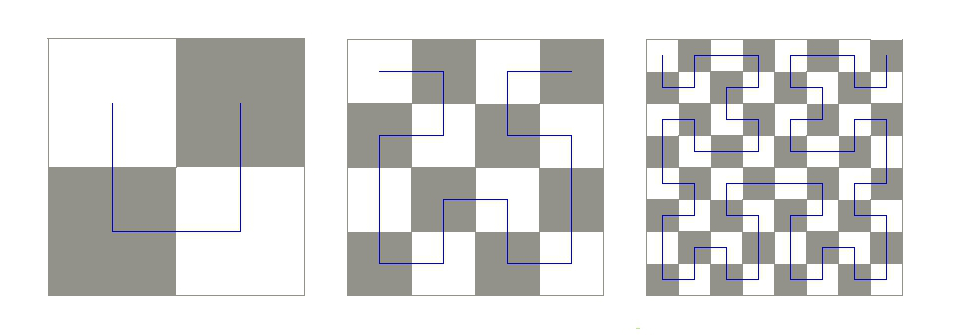
\includegraphics[width=.95\linewidth]{img/02/courbe_Hilbert.jpeg} 
        \caption[Courbe de Hilbert]{Principe de la courbe de Hilbert. 
        %http://www.lifl.fr/~pmathieu/transform/fractales.html
 		\label{fig:hilbert}}
\end{figure}

%
%\begin{figure}[bth]
%        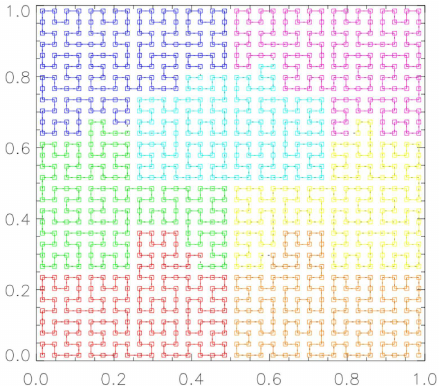
\includegraphics[width=.95\linewidth]{img/02/hilbert2.png} 
%        \caption{exemple de courbe de Hilbert. 
%%http://iopscience.iop.org/article/10.1086/590370/pdf 
%}
% 		\label{fig:hilbert2}
%\end{figure}

Dans l'état actuel de EMMA, la courbe est calculée au début de la simulation, et seule la grille coarse est prise en compte.
La répartition des domaines est statique et n'évolue pas au cours de la simulation.
Dans le cas ou un domaine raffine plus qu'un autre, la charge de travail y est plus importante.
Dans le futur, l'objectif serait de calculer la courbe de Hilbert sur la totalité des cellules feuilles.
Pour ainsi pouvoir refaire le découpage et équilibrer la charge entre les processeurs, et réaliser un "load balancing".

\subsection{Les domaines}

Chaque processus dispose d'un domaine de calcul correspondant à une sous partie de la grille.
Cependant, les domaines doivent communiquer entre eux et doivent être sensible a la structure \ac{AMR} de leurs voisins.
Pour répondre à ce problème, EMMA utilise le "Local essential tree decomposition" \citep{Warren:1993:PHO:169627.169640}.
Chaque processus dispose d'une vue globale de toute la grille ( cf Fig. \ref{fig:domaine}) mais la partie de la grille qui n'appartient pas au processeur est vue a résolution dégradée.
Ceci facilite grandement le gestion des conditions de bords.

\begin{figure}[bth]
        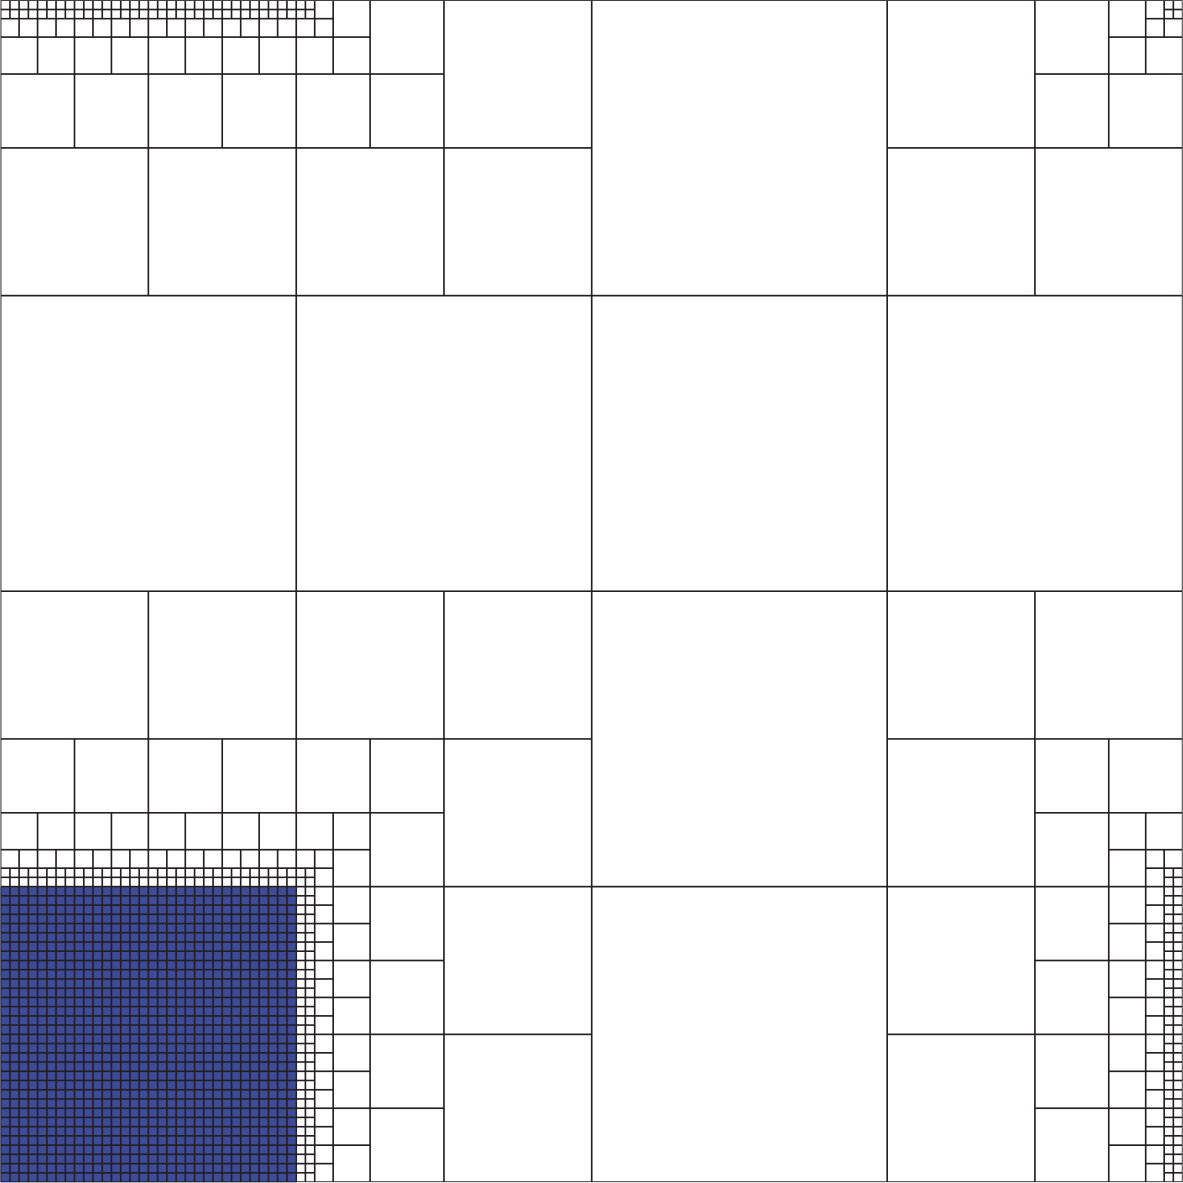
\includegraphics[width=.95\linewidth]{img/02/secteur.png} 
        \caption[Domaine associé a un processus]{Exemple de domaine de processeur généré par EMMA. 
        Chaque domaine représente une vue d'ensemble de la grille, a résolution dégradée.
}
 		\label{fig:domaine}
\end{figure}

\subsection{GPU}

EMMA utilise un degré supplémentaire de parallélisation.
Les calculs de chaque domaines sont accéléré en utilisant les capacités parallèle des processeurs graphiques récents.
Les cartes graphiques, ou \ac{GPU} ont été détourné de leurs utilisation principale d'affichage il y a une dizaine d'années et offre une capacité de parallélisation importante. 

A l'inverse des \ac{CPU} actuels qui disposent d'un nombre réduit de cœurs, les \ac{GPU} disposent d'une nombre beaucoup plus important de cœurs.
Par exemple un AMD Opteron 6300 de TITAN dispose de 16 cœurs, contre 2880 cœurs pour une NVIDIA Tesla k40c.
Un  \ac{CPU} peux exécuter des taches différentes sur chacun de ses cœurs (MIMD) tandis ce que les \ac{GPU} utilise un mode de parallélisation de type SIMD (Fig \ref{fig:cpugpu}).
Ce mode de parallélisation en font des unités de calculs efficaces dans le traitement d'un grand nombre d'informations en parallèle.
Elle sont donc toutes indiqués dans le cas des simulations numérique ou il s'agit d'appliquer un traitement identique à un grand nombre de cellules.

\begin{figure}[bth]
        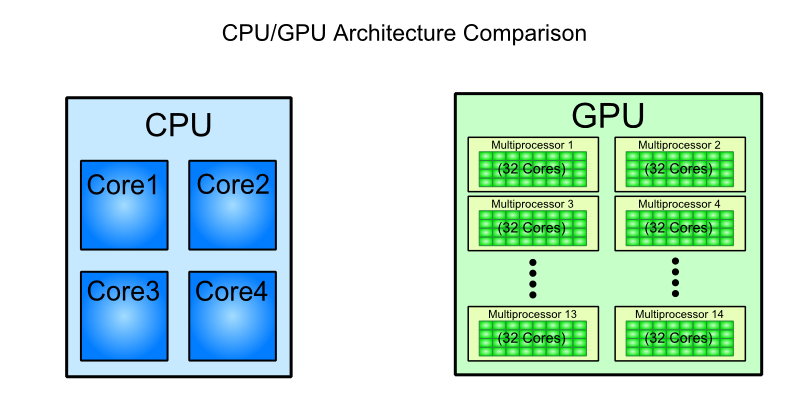
\includegraphics[width=.95\linewidth]{img/02/cpu_vs_gpu.png} 
        \caption[Comparaison CPU/GPU]{Comparaison CPU/GPU. Un \ac{CPU} dispose d'un nombre réduit de cœurs capables d’exécuter des opération complexe. 
        A l'inverse un \ac{GPU} dispose d'un grand nombre de cœurs pouvant exécuter un grand nombre d'opérations simples en parallèle}
 		\label{fig:cpugpu}
\end{figure} 

De plus, il existe au niveau matériel, deux avantages des \ac{GPU} par rapport aux \ac{CPU}.
Premièrement leurs meilleurs ratio puissance de calcul sur coup (flop/€).
Et également un meilleur ratio puissance de calcul sur puissance électrique (flop/W) ce qui réduit les besoins de refroidissement et permet des économies supplémentaires.

Cependant \ac{CPU} et \ac{GPU} sont indissociables est doivent être utilisé conjointement pour tirer le meilleurs parti des capacités de calcul offerte par une machine hybride.
La programmation sur carte graphique utilise une approche proche du concept de mémoire distribuée, c'est à dire que leurs espaces mémoire ne sont pas commun.
Une code hybride est découpé en deux parties, une partie séquentielle exécutée sur le \ac{CPU} et une partie parallèle exécutée sur le \ac{GPU}.
Le passage de \ac{CPU} à \ac{GPU} va donc nécessiter des communications.

%On tirera le maximum des capacités d'accélération d'un \ac{GPU} avec un code qui est hautement parallélisable.

%Il faut donc que la quantité de calcul effectués par la carte soit suffisante pour rentabilisé la communication.
%plus dur a programmer, performance dépends du problème.


%Or a l'heure actuelle cette communication utilise une interface relativement lente (PCI express) qui rend coûteuse la communication. 

% et de 12Go de mémoire et a une puissance de calcul de 4.3 Tflop/s en simple precision.
%
%
%Intel® Xeon® X7560 -> TDP 130 W -> 76 Gflop/s (crete)
%
%
%IBM A2 (sequoia) -> 204 Gflop/s -> TDP 55W


\subsection{Les communications CPU/GPU}
\label{sec:cpugpu}

Les \ac{CPU} sont capable d'accéder rapidement aux informations en mémoire, quel que soient leurs organisations.
Le \ac{GPU} sont quant à eux sensibles à la segmentation des données.
C'est à dire que les calculs sur ac{GPU} seront plus performants si les données sont organisées de façons à ce que leurs accès mémoire consécutifs soient physiquement proches.
%Prenons l'exemple d'une différence finie. 
%Pour calculer le nouvel état d'une cellule, il est nécessaire de connaitre sont état actuel, et celui de sa voisine.
%L'accès mémoire sera plus rapide si l'information est situer sur un espace mémoire adjacent.
%Ce choix est motivé par le fait qu'une structure mémoire bien organisée peux amener a des gains conséquents.
Par exemple dans CUDATON \citep{aubert_radiative_2008} un code de transfert radiatif sur grille fixe, le gain de la parallélisation GPU est de l'ordre de 80 car la structure mémoire est optimisée.

La difficulté est que l'arbre \ac{AMR} ne respecte pas cette organisation, et la mémoire peut être extrêmement fragmentée à cause de la liste chainée.
Pour limiter l'impact de la fragmentation, le choix a été fait d'organiser les données sur le CPU, avant de les envoyer dans l'espace mémoire du GPU.
Cette opération sera appelée "gather" (cf Fig. \ref{fig:gatherscatter}).
Les données organisées sont envoyés sur le GPU, pour effectuer les calculs.
Le résultat est ensuite copié sur le CPU et remises dans l'arbre par le CPU (opération de "scatter").
Dans le cas où les calculs sont réalisés sur le CPU, cette opération est quand même réalisée, dans le but de conserver une certaine cohérence entre les versions.

\begin{figure}[bth]
        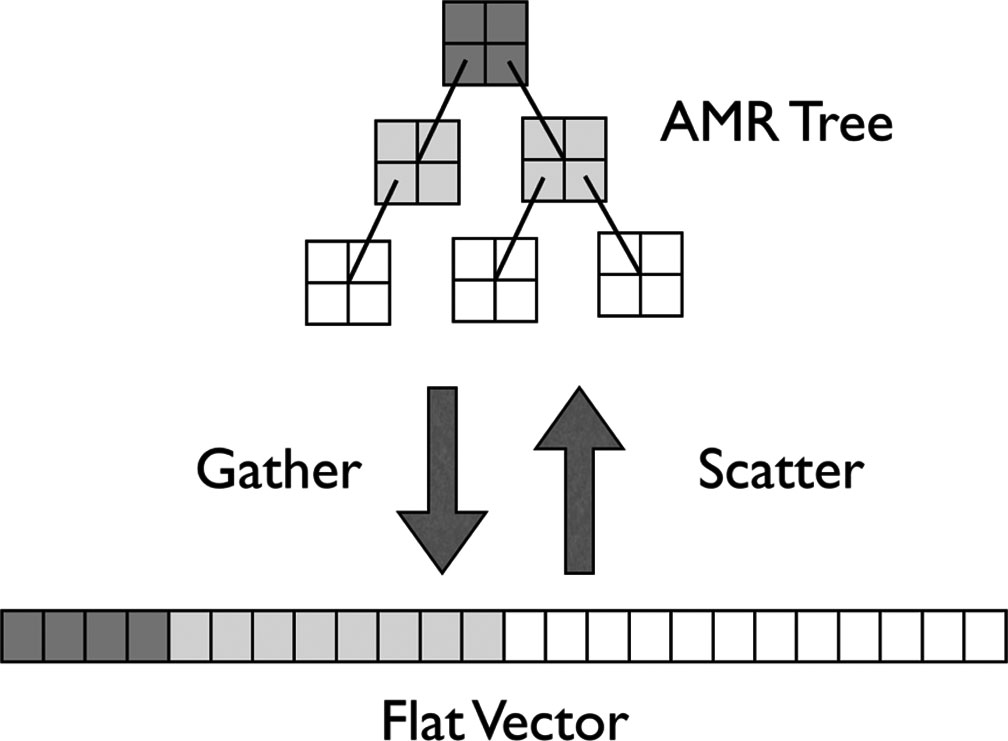
\includegraphics[width=.95\linewidth]{img/02/gatherscatter.jpg} 
        \caption[Passage AMR / vecteur]{Transition entre la structure en arbre de l'AMR et la structure en vecteur de calcul.
        L'arbre est sur le CPU, le vecteur est sur le GPU.
 		\label{fig:gatherscatter}
 		}
\end{figure}

Le pari est ici que la perte de temps générée par les opérations de gather/scatter sera compensé par l'accélération du GPU.

En pratique l'opération de gather consiste a rassembler toutes les informations nécessaire au calcul de l'état d'une cellule.
Par exemple pour le calcul du potentiel (cf sec. \ref{sec:gravity}) les données nécessaires seront: la densité locale, le potentiel local, le potentiel des 6 cellules voisines suivant les axes principaux.
Ces données sont rassemblées dans une structure, puis une série de structure est stockée dans un tableau.
Cette opération sera réalisée par paquet de $N$ cellules pour chaque cellule de la grille.

On peut observer ici que les copies ont beaucoup de redondance.
la copie est composé d'une cellule centrale et des 6 cellules voisine le ratio information utile sur information nécessaire est de $1/6$..
En passant à la cellule suivante, la cellule précédente sera de nouveau copiée et au final le potentiel d'une cellule sera donc copié sept fois sur le GPU.
Ces multiples copies diminue grandement les performances et en font l'une des principales limitations à l'accélération globale du code.
Toute fois, même dans cet état, l'exécution s'en trouve accélérée d'un facteur $\approx 3$ par rapport à la version CPU.

Dans le but de réduire le nombre de copies et accélérer l'exécution du code, j'ai modifié les opérations de gather/scatter pour diminuer la redondance des copies.
Au lieu de traiter les cellules unes par unes, l'idée est de traiter les octs.
Dans ce cas les cellules sont traitées par 8 et les voisinages au sein d'un oct n'ont pas besoin d'être copiés plusieurs fois.
On copie donc 8 cellules d'intérêt et 4 cellules de bord par face du cube, soit 24 cellules.
Le ratio utile/nécessaire passe donc à $8/24 = 1/3$.
La quantité de copies redondante a donc été divisé par 2 par rapport au cas précédent.

Vu que la surface d'un cube augmente avec le carré de son coté, alors que son volume augmente avec son cube, plus grand sera la nombre de cellule d'intérêt, meilleur sera la ratio.
En étendant ce principe, j'ai développé une méthode qui permet de manière récursive d'envoyer une portion d'AMR contenue dans un OCT de niveau arbitraire.
Cependant les résultats ne sont pas a la hauteur des espérances, et l'accélération n'est pas proportionnelle au ratio de données utiles.

IL existe cependant des pistes pour améliorer ce goulot d'étranglement.
Une possibilité est de séparer la gestion de l'arbre de la physique.
En l'état actuel, les données physique sont stockées en mémoire avec la même structure que l'arbre.
L'idée serait de stocker dans l'arbre, des indices de cellules permettant de retrouver l'information physique dans des vecteurs plat (cf Fig. \ref{fig:gatherscatter}).
Ainsi les vecteurs pourraient être en permanence sur le GPU, et seul l'information sur leurs position dans l'AMR devrait être transmise.
Un grand nombre de copies seraient alors évitées. 

Une autre possibilité serait de placer l'intégralité de l'arbre sur le GPU.
Dans ce cas, toutes les copies seraient supprimées mais c'est le GPU qui devra gérer l'évolution de l'arbre. 
Il existe des techniques optimisé de gestion d'arbre sur GPU à base de "Z-order curves", mais son implémentation nécessite une refonte en profondeur du code.

%optimisation matérielle -> les prochaines générations de GPU


%est de séparer la gestion de l'arbre de la physique.
%La plus prometteuse semble être de supprimer complètement les copies en plaçant la totalité de l'arbre directement sur la carte.
%Le CPU étant tres efficace pour ce genre d'opération, il semble

%Copies asynchrones

\subsection{Gestion des entrées sortie}

Durant ma thèse la simulation CODA II EMMA (voir partie \ref{sec:CODAEMMA}) a été réalisée.
Cette simulation fait partie des plus grosse simulation de la réionisation exécutée à l'heure actuelle avec un nombre de particules de matière noire, et donc une grille de base, de $2048^3$ éléments .
Ces données devront être stockées et écrites sur disque dur or si l'on se réfère à la table \ref{tab:debits} on observe que les débits d'accès disques sont les plus faibles.

Pour se faire une idée de la quantité de données en jeu faisons une estimation : 

\begin{itemize}
\item Pour les particules:
En considérant qu'un flottant est codé sur 4 octets, chaque champs représente $2048^3 \cdot 4 = 32$Go.
Comme il y a une dizaine de champs en sortie (3 positions, 3 vitesses, etc) les particules représentes environs $320$Go.

\item Pour la grille :
En considérant que la quantité de cellule peut être multipliée par 3 à cause du raffinement, chaque champ (densité, température, composante de la vitesse, etc..) représente environ $32 \cdot 3 \approx 100$Go.
Il y a au total un cinquantaine de champs calculés à l'exécution de la simulation mais en pratique environ une vingtaine en sortie.
Chaque écriture de la grille représente donc $100\cdot 20 =2$To.

\item Pour les étoiles:
C'est très variable car dépend directement du nombre d'étoile à l'instant donné, qui dépend lui même du paramètre de résolution en masse.
\end{itemize}

Ce qui représente au total environ 2,3 To de données générée par pas de temps de sortie.
Mais on voudrait évidemment avoir accès a l'état de la simulation à différents instant, cette simulation a au final générée 170 snapshot.
Au final le volume de donnée de la simulation représente près de 400 To.
%De plus, ces données sont stockées sur \ac{HDD}, et si l'on se réfère à la table \ref{tab:debits} on observe que les débits d'accès disques sont les plus faibles.
Étant donné la quantité de données en jeu, une bonne gestion des Entrées/Sorties peut donc permettre un gain de temps appréciable.
De plus, ces données sont généralement calculé sur des machines distante et améliorer leur compacité peut permettre de gagner du temps au moment du transfert vers des machines locales, ou simplement au moment de la lecture pour analyse.

%Les entrées/sorties sont des étapes relativement longues et l'écriture sur disque d'une telle quantité de données demande du temps et ralentit l'exécution de la simulation.
% leurs rapatriement sur des machine locales peut également être coûteux en temps.
%Il a fallu plusieurs mois pour rapatrier localement les données générées par la simulation CODA.
%Il a fallut plusieurs mois pour rapatrier les données de CODA de TITAN aux états unis vers Strasbourg
%De plus améliorer la compacité des données permet également de gagner du temps au moment du transfert vers des machines distante, ou simplement au moment de la lecture
%analyse a distance
%le feedback CODA\\
%grosse quantité de données\\

Dans l'ancien modèle de données d'EMMA, l'intégralité de l'octree était écrit (cf figure \ref{fig:data}).
Les octs étaient écrit les uns à la suite des autres avec toute l'information qu'ils contenaient.
L'information étaient exacte et complète, mais le volume de données était considérable.
De plus chaque processeur écrivait un fichier indépendant, ce qui pouvait rapidement faire exploser le nombre de fichiers et être problématique selon file-système des calculateurs car il est possible d'avoir un nombre limité de fichier par utilisateur.

Dans la même optique que ce qui a été abordé dans la section \ref{sec:cpugpu}, j'ai mis en place un modèle visant a manipuler les données avant leurs transferts.
L'objectif est de sortir les données de l'arbre en se basant sur une notion de tableau de champs pour faciliter leurs traitement.
Dans ce nouveau modèle, seules les feuilles (les cellules non raffinées) sont écrites sur le disque, ce qui permet de réduire le volume et la redondance des données.

Les champs sont maintenant traités individuellement (cf figure \ref{fig:data}) et il est possible de choisir de les écrire ou non en fonction des besoins.
Les champs sont séparés dans des fichiers distincts, et les processeurs écrivent conjointement dans le même fichier grâce a l'utilisation de la librairie hdf5.
Le nombre total de fichiers ne dépend plus du nombre de processeurs sur lequel a tourné la simulation.
Et lors d'un transfert entre machine, il est possible de ne rapatrier que les données nécessaire, et ainsi économiser du temps et de la bande passante.

Malgré la quantité de données réduite, le temps passé dans la fonction de sortie n'en est que très peu affecté.
Le gain réalisé au moment de l'écriture est compensé par la charge de calculs supplémentaires due à l'extraction des données de l'arbre.
Par contre un gain appréciable est réalisé au moment de l'analyse des données.

\begin{figure}
        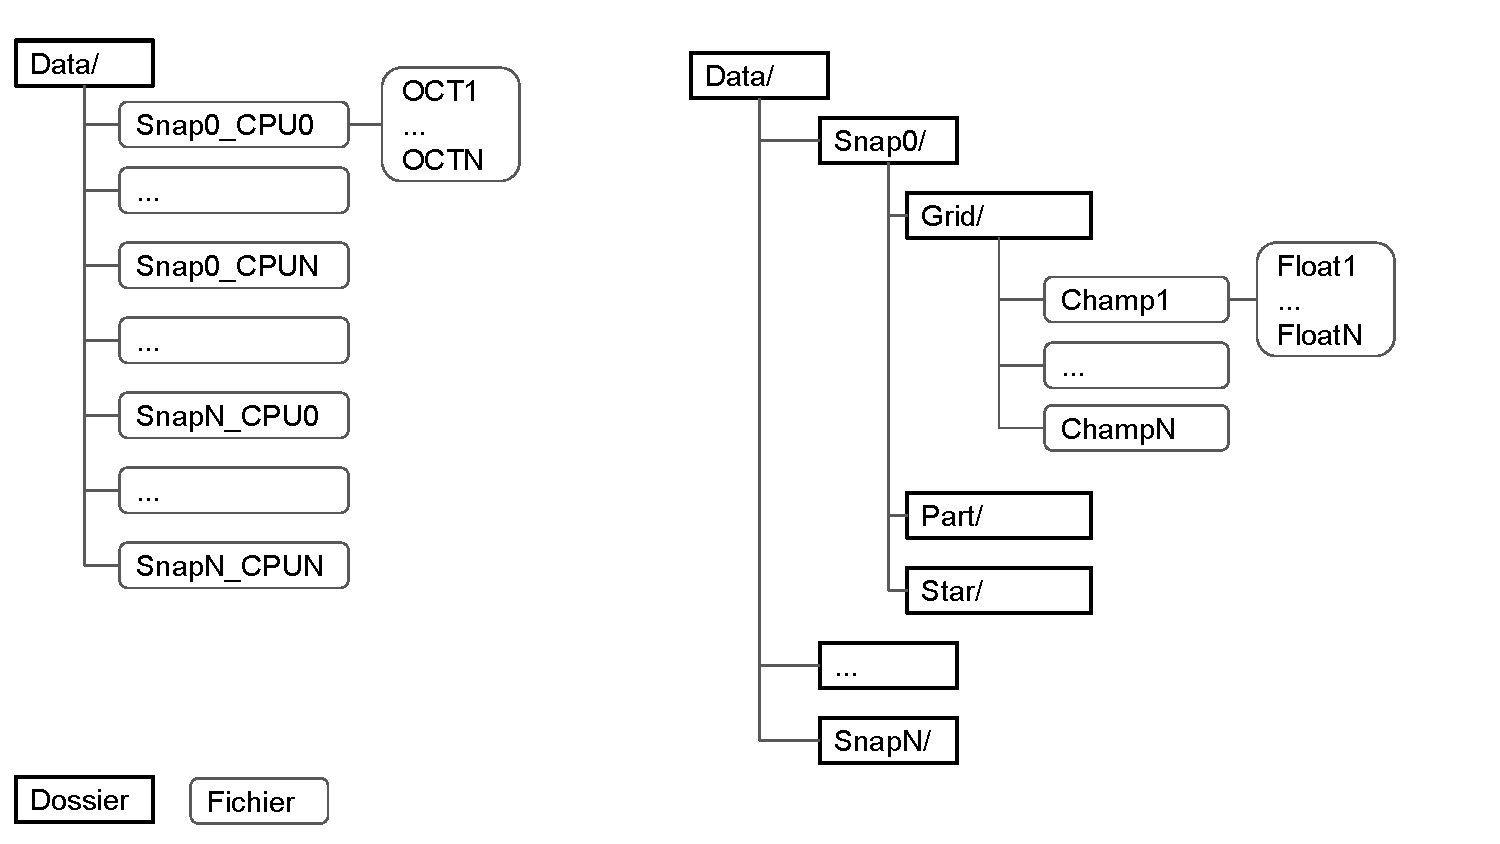
\includegraphics[width=.95\linewidth]{img/02/data.pdf} 
        \caption[Gestion des IO]{Différence entre ancienne gestion des données à gauche et nouvelle version à droite.
 		\label{fig:data}
 		}
\end{figure}


%En contrepartie, il est nécessaire de reprojeter la grille dans le cas d'une analyse sur un niveau intermédiaire.

%Chaque cellule est considérée comme une particule d'une certaine taille.

%Architecture des données 
%conception d'une organisation des données
%séparation des champs
%structure imposé par la gestion de l'AMR
%écriture parallèle

%\subsection{Potentiel d'optimisation EMMA}
%
%la forme des gathers/scatter
%optimisation matérielle -> les prochaines générations de GPU
%Opérations coarse sur grille non AMR.
%reformatage de l'arbre et découplage de la physique


%\begin{figure}[bth]
%        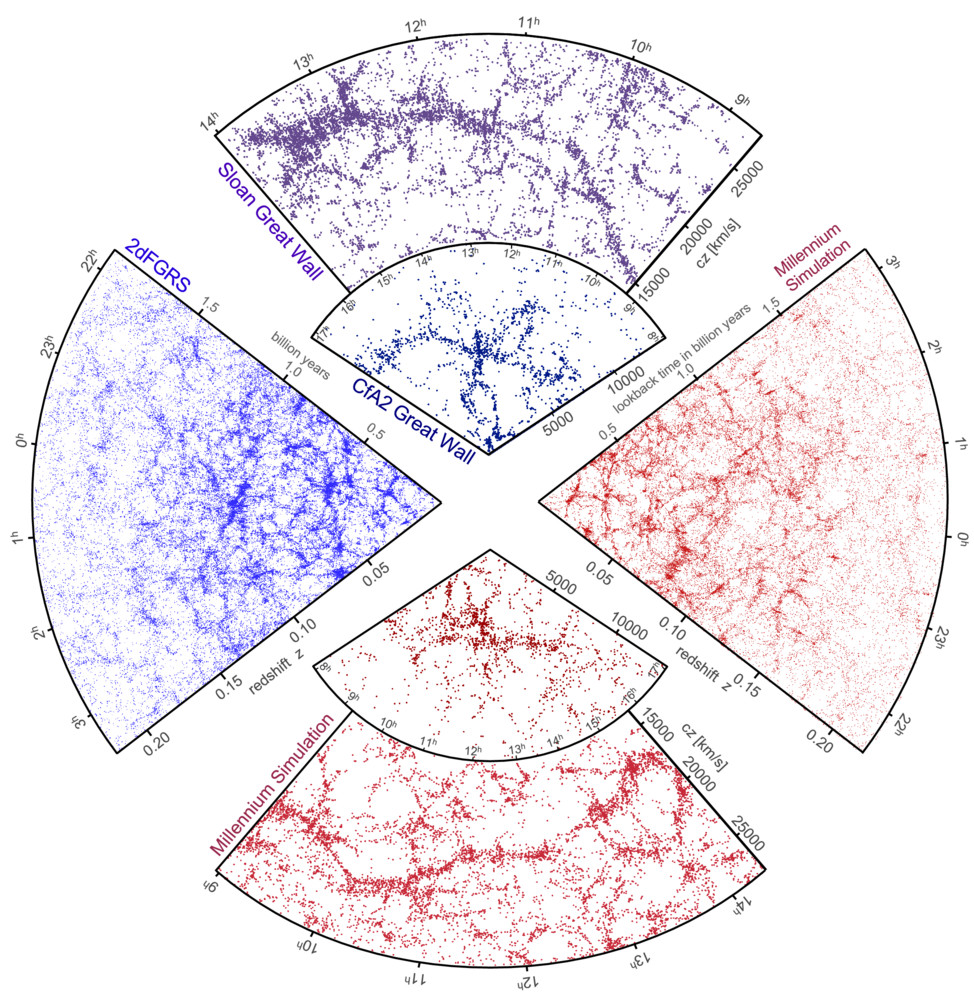
\includegraphics[width=.95\linewidth]{img/02/sdss_millenium.jpeg} 
%        \caption{ 
%%http://wwwmpa.mpa-garching.mpg.de/millennium/
%}
% 		\label{fig:}
%\end{figure}
